\section{Abstract model for DAE units}

\begin{defn}
	Let us define $\myatam$ (DAE $\atam$) as $\atam$ where
	\begin{itemize}
		\item temperature is set to $\tau = 2$,
		\item there are another $5$ tile shapes\footnote{Even with their vertical reflections.}, see Figure \ref{fig:abstract_model} (tiles {\sf ADEB}, {\sf CA}, {\sf KG}, {\sf KLO} and {\sf OP DONE}),
		\item initial tile $t_0$ is set to the left bottom tile (in Figure \ref{fig:abstract_model} tile {\sf CA}),
		\item glue strengths are restricted to corresponding tile type, all of which appear in Figure \ref{fig:abstract_model}.
	\end{itemize}
\end{defn}

\begin{note}
	$\myatam$ can be easily simulated by classical $\atam$ at temperature $2$.
\end{note}

Those bottom tiles have side glue strengths $2$ thus they can form a linear sequence\footnote{Note that the word can be restricted by arbitrary regular grammar rule.}. This sequence plays the role of the seeked certificate from Definition \ref{def:NP}. Then the other tiles ``check'' correctness of this certificate with polynomial complexity. Note that binding complexity is related to probability of error thus we will be interested even in constants, see example in Remark \ref{rem:tilde}.

%!% odhady se dají zmenšit pomocí #E místo #V^2

\begin{figure}[H]
\begin{center}
	\begin{subfigure}[b]{0.31\textwidth}
		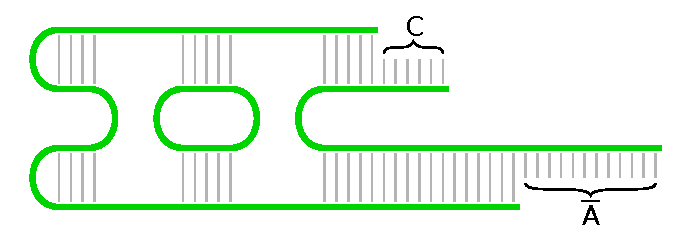
\includegraphics[width=\textwidth]{./figures/tile_model/DNA_struct.pdf} % 115mm
		\caption{Corner DAE unit}
		\label{fig:DNA_struct}
	\end{subfigure}
	\begin{subfigure}[b]{0.472\textwidth}
		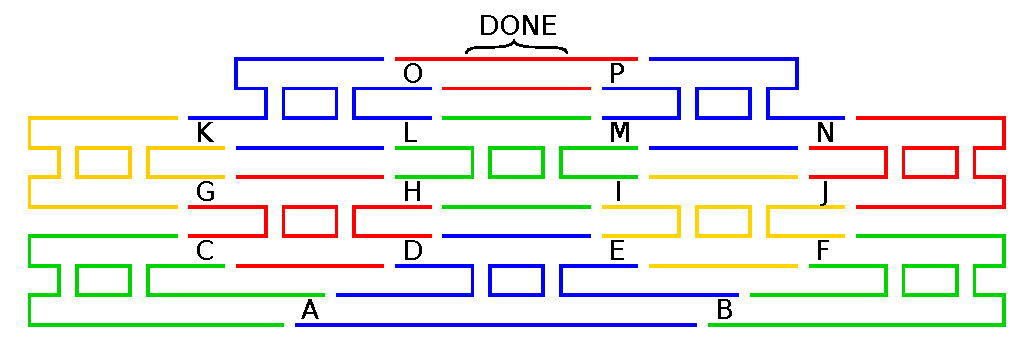
\includegraphics[width=\textwidth]{./figures/tile_model/DNA_assembly.pdf} % 175mm
		\caption{Scheme of self-assembly}
		\label{fig:DNA_assembly}
	\end{subfigure}
	\begin{subfigure}[b]{0.190\textwidth}
		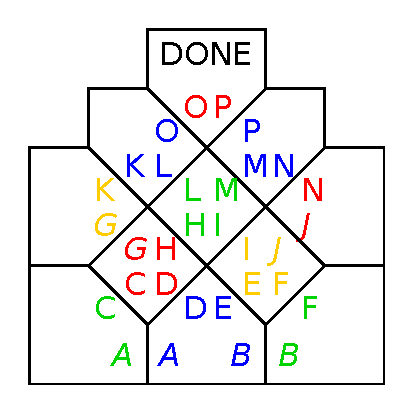
\includegraphics[width=\textwidth]{./figures/tile_model/abstract_model.pdf} % 70mm
		\caption{Abstract model}
		\label{fig:abstract_model}
	\end{subfigure}
	\caption{Evolution of $\myatam$ model from DAE units to tiles. Here italic glues {\sf A}, {\sf B}, {\sf G} and {\sf J} are of strength $2$.} %!% okomentovat že se nic neposere těma lepidlama = 2 na krajích
	\label{fig:evolution}
\end{center}
\end{figure}
